\documentclass[fr,license=none]{../../../eplsummary}

\usepackage{array}
\usepackage{fancybox}
\usepackage{float}
\usepackage{colortbl}
\usepackage{makecell}
\usepackage{graphicx}
\usepackage{titlesec}
\usepackage{qtree}
\usepackage{tensor}
\usepackage{circuitikz}

\usepackage{../../../eplelec}
\usepackage{../../../eplunits}

\hypertitle[']{\'Electricit\'e}{1}{FSAB}{1201}
{Nicolas Cognaux\and Mattéo Couplet\and Guillaume Fran\c{c}ois\and Beno\^it Legat}
{Jean-Didier Legat}

\part{Électrostatique}
\section{Champ électrique et charge électrique}

Deux charges de même signe se repoussent.
Deux charges de signes opposés s'attirent.

\subsection{Loi de Coulomb}
L'intensité de cette force vaut
\[ |F| = \frac{1}{4\pi\perm_0}\frac{|q_1q_2|}{r^2} \]
avec $q_1$ et $q_2$ les charges respectives, $r$ la distance qui les sépare et $\perm_0$ la permittivité du vide
\[ \perm_0 \approx \SI{8.85e-12}{\coulomb\squared\per\newton\per\meter\squared} \]

On utilise aussi parfois
\[ k \eqdef \frac{1}{4\pi\perm_0} \approx
\SI{9e9}{N.m^2/C^2} \]

\subsection{Champ électrique}
Le champ électrique est la force électrostatique par unité de charge
\[ \vec{E} = \frac{\vec{F}}{q} \]
Le champ électrique $\vec{E}$ causé par une charge $q$ située à une distance $r$ peut donc être réécrit comme suit
\[ \vec{E} = \frac{1}{4\pi\perm_0}\frac{q}{r^2}\hat{r} \]
$\hat{r}$ est le vecteur unitaire pointant radialement vers l'extérieur.
L'amplitude de $\vec{E}$ en un point peut être vue comme la force que subirait une charge de $\SI{+1}{\coulomb}$ en ce point. \\\
\begin{tabular}{ll}
  Champ d'un point de charge & \(\frac{1}{4\pi\perm_0}\frac{q}{r^2}\)\\
  Champ à  l'extérieur d'une sphère &
  \(\frac{1}{4\pi\perm_0}\frac{Q}{r^2}\)\\
  Champ à  l'intérieur d'une sphère &
  \(\frac{1}{4\pi\perm_0}\frac{Qr}{R^3}\)\\
  Champ d'une plaque infinie & \(\frac{\sigma}{2\perm_0}\)\\
  Champ entre deux plaques de charges opposées & \(\frac{\sigma}{\perm_0}\)
\end{tabular}

\subsection{Lignes de champ électrique}
Les lignes de champ électrique partent
de la charge positive et vont vers la charge négative.
\begin{itemize}
  \item Elles ne s'intersectent jamais;
  \item Leur nombre donne une idée de l'intensité du champ électrique;
  \item Le champ électrique est tangent aux lignes de champ électrique.
\end{itemize}

\section{Dipôles}
Un dipôle électrique est une paire de charges électriques de même amplitude $q$ mais de signes opposés, séparés par une distance $d$. Le moment $\vec{p}$ du dipôle, orienté de la charge négative à la charge positive, a une amplitude $p=qd$. Dans un champ électrique $\vec{E}$, le dipôle subit un moment de force
\[ \vec{\tau} = \vec{p} \times \vec{E} \]
L'énergie potentielle vaut
\[ U = -\vec{p} \cdot \vec{E} \]

\section{Flux électrique et loi de Gauss}
Le flux électrique mesure la quantité de champ électrique passant à travers une surface.
\[ \Phi_E = \int \vec{E} \cdot \dif\vec{A} =
\int E_{\perp} \dif A = \int E\cos\phi \, \dif A \]

\subsection{Loi de Gauss}
Si ce flux $\Phi_E$ est calculé sur une surface fermée,
alors il vaut la somme des charges à l'intérieur
de cette surface fermée divisée par $\perm_0$
\[ \oint \vec{E} \cdot \dif\vec{A} = \frac{Q_\mathrm{encl}}{\perm_0} \]

\subsection{Application}
Pour les conducteurs, les charges sont à la surface,
soit $\sigma$ la quantité de charge par unité de surface, on a par Gauss
\[ \oint E_\perp \dif A = \frac{\sigma A}{\perm_0} \]
Si la forme du conducteur est suffisamment symétrique
pour que $E_\perp$ soit constant, on a donc
\[ E_{\perp} = \frac{\sigma}{\perm_0} \]

\section{Énergie potentielle électrique}
Le travail que doit effectuer une charge pour se rendre de $a$ à $b$ est égal à la différence de potentiel électrique entre ces deux points
\[ W_{a\rightarrow b} = U_a - U_b = -\Delta U = \int_{a}^{b} \vec{F} \cdot \dif \vec{l} \]
Dans le cas d'une charge $q_0$ se déplaçant sous l'effet d'une charge $Q$, on a
\[ W_{a\rightarrow b} 
    = \int_{a}^{b} \vec{F} \cdot \dif \vec{l}
    = \int_{r_a}^{r_b} F \dif r
    = \int_{r_a}^{r_b}\frac{1}{4\pi\perm_0}\frac{Qq_0}{r^2} \dif r
    = \frac{Qq_0}{4\pi\perm_0}\left(\frac{1}{r_a} - \frac{1}{r_b}\right) \]

Ainsi, l'énergie potentielle que possède une charge $q_0$ en présence d'une autre charge $q$ vaut, à une constante près,
\[ U = \frac{1}{4\pi\perm_0} \frac{qq_0}{r} \]
De manière générale, l'énergie potentielle en présence d'un ensemble de charges vaut, à une constante près,
\[ U = \frac{q_0}{4\pi\perm_0} \sum_i \frac{q_i}{r_i} \]

\section{Potentiel électrique}
Le potentiel électrique est l'énergie potentielle par unité de charge
\[ V \eqdef \frac{U}{q_0} \]
La différence de potentiel entre deux points représente le travail que doit effectuer une charge de \SI{+1}{\coulomb} pour se mouvoir entre ces points.

\begin{tabular}{ll}
    Potentiel dû à une charge ponctuelle & $\frac{1}{4\pi\perm_0} \frac{q}{r}$ \\
    Potentiel dû à un ensemble de charges & $\frac{1}{4\pi\perm_0} \sum_i \frac{q_i}{r_i}$ \\
    Potentiel dû à une distribution de charge & $\frac{1}{4\pi\perm_0} \int\frac{\dif q}{r}$
\end{tabular}

On peut également calculer une différence de potentiel en intégrant le champ électrique
\[ V_{ab} = V_a - V_b = \int_{a}^{b}\vec{E}\cdot\dif\vec{l}
= \int_{a}^{b}E\cos{\phi} \dif l \]
Inversement, le champ électrique en un point est le gradient du potentiel électrique en ce point
\[ \vec{E} = - \grad V \]

\section{Capacités et diélectriques}
Une capacité est une paire de conducteurs séparés par un isolant. Lorsqu'elle est chargée, chaque conducteur possède une charge opposée de même amplitude $Q$, proportionnelle à la différence de potentiel entre les conducteurs
\[ Q = CV \qquad C = \perm_0\frac{A}{d} \]
Capacité équivalente
\begin{description}
    \item[en série] $\frac{1}{C_\text{éq}} = \sum_i \frac{1}{C_i}$
    \item[en parallèle] $C_\text{éq} = \sum_i C_i$
\end{description}

L'énergie stockée dans une capacité vaut
\[ U = \frac{1}{2}CV^2 = \frac{Q^2}{2C} = \frac{1}{2}QV \]
La densité énergétique (énergie par unité de volume) vaut
\[ u = \frac{1}{2} \perm_0 E^2 \]

L'insertion entre les conducteurs d'un matériau diélectrique augmente la capacité d'un facteur $K$, appelé constante diélectrique du matériau
\[ \perm = K \perm_0 \qquad C = KC_0 = \perm \frac{A}{d} \qquad V = \frac{1}{K}V_0 \]
\[ u = \frac{1}{2} \perm E^2 \]

Loi de Gauss dans un diélectrique ($Q_\text{encl-free}$ n'inclut que les charges libres)
\[
    \oint K\vec{E} \cdot \dif\vec{A} = \frac{Q\text{encl-free}}{\perm_0}
\]

\newpage
\part{Courant continu (DC)}
%      ___
%  ___(- +)___
% |    ---    |
% |    ELEC   |
% |_____||____|
\section{Courant et densité de courant}
\[ I = \fdif{q}{t} = n q v_d A \qquad{\qquad{\qquad}}\rho =
% Je suppose que n|q|v_dA signifie l'expression ci-dessus.
\frac{E}{J} \qquad{\qquad{\qquad}} q(t) = \int_{t_0}^{t}i(t) \dif t + q(t_0) \]
$J$ est la densité de courant : $J = \frac{I}{A}$.

\section{Résistance et résistivité}
\[ R = \frac{\rho{L}}{A} \qquad{\qquad{\qquad}}V = IR \]

Résistance équivalente
\begin{description}
    \item[en série] \( R_\text{éq} = \sum_i{R_i} \)
    \item[en parallèle]  \( \frac{1}{R_\text{éq}} = \sum_i{\frac{1}{R_i}} \)
\end{description}

\section{Force électromotrice et puissance}
\[ P = VI = RI^2 = \frac{V^2}{R} \] 
\[ V_{ab} = \EMF - IR_\text{interne}\qquad{\qquad{\qquad}}w
= \int_{t_1}^{t_2}p(t) \dif t \]

\section{Lois de Kirchhoff}
\begin{description}
    \item[dans un nœud] \( \sum{I} = 0 \)
    \item[dans une boucle] \( \sum{V} = 0 \)
\end{description}

\section{Équivalents de Thévenin et de Norton}

Tout circuit composé de sources de courant ou de tension et de résistances peut être remplacé par une source de tension et une résistance en série (équivalent de Thévenin) ou par une source de courant et une résistance en parallèle (équivalent de Norton).

% TODO: bien positionner les circuits
\begin{center}
\begin{tabular}{cc}
    Équivalent de Thévenin & Équivalent de Norton \\
    \begin{circuitikz}[american]
        \draw (0, 0)
            to[short, -o] (2, 0)
            to[open, v<=$V_\mathrm{co}$] (2, 2)
            to[R=$R_\mathrm{éq}$, o-] (0, 2)
            to[V, v_=$V_\mathrm{th}$] (0, 0)
        ;
    \end{circuitikz}
    & 
    \begin{circuitikz}[american]
        \draw (0, 0)
        to[I, i=$I_\text{n}$] (0, 2)
        to[short] (1, 2)
        to[R=$R_\text{éq}$] (1, 0)
        to[short] (0, 0);
        \draw (1, 0) 
        to[short, -o] (2, 0)
        to[open] (2, 2)
        to[short, o-] (1, 2);
    \end{circuitikz}
\end{tabular}
\end{center}

La tension de Thévenin est la tension en circuit ouvert aux bornes. Le courant de Norton est le courant en court-circuit dans la branche entre les bornes.
\[ 
    V_\text{Thévenin} = V_\text{circuit ouvert} \qquad
    I_\text{Norton}   = I_\text{court-circuit}
\]

Les résistances de chacun des circuits sont équivalentes. Il vient donc
\[ V_\text{Thévenin} = R_\text{équivalente} \cdot I_\text{Norton} \]

Dans le cas où les sources de courant et de tension dans le circuit sont toutes indépendantes (non contrôlées), la résistance équivalente vaut la résistance équivalente du circuit en supprimant toutes les sources (les sources de tension (resp. de courant) deviennent des court-circuits (resp. des circuits ouverts)).

Si des sources contrôlées sont présentes, il faut impérativement calculer $V_\text{th}$ et $I_\text{n}$ séparément pour connaitre $R_\text{éq}$.

\section{Capacités et inductances}
\begin{table}[H]
  \begin{center}
    \begin{tabular}{|m{6.5cm}|m{6.5cm}|}
      \hline
      \multicolumn{1}{|c|}{\textbf{Capacité}} &
      \multicolumn{1}{c|}{\textbf{Inductance}}\\
      \hline
      \[ I(t) = C\fdif{V}{t} \] & \[ V(t) = L\fdif{I}{t} \]\\
      \[ U = \frac{CV^2}{2} = \frac{Q^2}{2C} \] & \[ U = \frac{LI^2}{2} \]\\
      \hline
      \multicolumn{1}{|c|}{\textbf{Circuit R-C}} &
      \multicolumn{1}{c|}{\textbf{Circuit R-L}}\\
      \hline
      \[ \tau = RC \] & \[ \tau = \frac{L}{R} \]\\
      \[ \fdif{V_{0-}}{t} = 0 \Rightarrow I_{0-} = 0 \]
      & \[ \fdif{I_{0-}}{t} = 0 \Rightarrow V_{0-} = 0 \]\\
      \[ U_{0-} = U_{0+} \Rightarrow V_{0-} = V_{0+} \]
      & \[ U_{0-} = U_{0+} \Rightarrow I_{0-} = I_{0+} \]\\
      \[ \fdif{V_{\infty}}{t} = 0 \Rightarrow I_{\infty} = 0 \]
      & \[ \fdif{I_{\infty}}{t} = 0 \Rightarrow V_{\infty} = 0 \]\\
      \[ V_{t>0}(t) = A + Be^{-t/\tau} \]
      & \[ I_{t>0}(t) = A + Be^{-t/\tau} \]\\
      \[ V_{0+} = A + B \] & \[ I_{0+} = A + B \]\\
      \[ V_{\infty} = A \] & \[ I_{\infty} = A \]\\
      \hline
    \end{tabular}
  \end{center}
\end{table}


\section{Circuit L-C}
Un circuit L-C est un circuit composé d'une capacité et d'une inductance en série.
\begin{center}
    \begin{circuitikz}[american]
        \draw (0, 0)
        to[L=$L$] (2, 0)
        to[short] (2, 2)
        to[C=$C$] (0, 2)
        to[short] (0, 0);
    \end{circuitikz}
\end{center}

On observe dans ce type de circuit une oscillation des charges entre les deux bornes de la capacité. La somme des énergies contenues par les composants étant supposée conservée, on a
\[ U_C + U_L = U_\mathrm{tot} \Leftrightarrow \frac{q^2}{2C} + \frac{LI^2}{2} = \frac{Q^2}{2C} \]
avec $Q$ la charge totale contenue dans le circuit.

Le courant passant à travers le circuit s'exprime donc
\[ I = \pm \sqrt{\frac{Q^2 - q^2}{LC}} \]
Notons qu'à chaque oscillation, le courant change de sens, d'où la présence du $\pm$.

En appliquant la loi de Kirchhoff sur l'unique boucle du circuit, on trouve la relation
\[ V_L + V_C = 0 \Leftrightarrow \frac{\dif^2 q}{\dif t^2} + \frac{1}{LC} q =  O\]
La solution générale de cette équation différentielle est de la forme
\[ q(t) = A \cos(\omega t + \phi) \]
En injectant cette solution dans l'équation, on trouve l'expression de la fréquence angulaire de l'oscillation
\[ \omega = \sqrt{\frac{1}{LC}} \]

\section{Circuit R-L-C}
Un circuit R-L-C est un circuit composé d'une capacité, d'une résistance et d'une inductance en série.
\begin{center}
    \begin{circuitikz}[american]
        \draw(0, 0)
        to[L=$L$] (2, 0)
        to[R=$R$] (2, 3)
        to[C=$C$] (0, 3)
        to[short] (0, 0);
    \end{circuitikz}
\end{center}
La résistance dissipe de l'énergie, l'énergie totale n'est donc pas conservée.

En appliquant la loi de Kirchhoff sur l'unique boucle du circuit, on trouve la relation
\[ V_R + V_L + V_C = 0 \Leftrightarrow \frac{\dif^2 q}{\dif t^2} + \frac{R}{L} \frac{\dif q}{\dif t} + \frac{1}{LC} q = 0 \]
La solution générale de cette équation différentielle est de la forme
\[ q(t) = A e^{kt} \cos(\omega t + \phi) \]
En injectant cette solution dans l'équation, on trouve l'expression de la fréquence angulaire de l'oscillation
\[ \omega = \sqrt{\frac{1}{LC} - \frac{R^2}{4L^2}} \]

\newpage
\part{Courant alternatif (AC)}
\begin{mynota}
  Quand le courant (resp. la tension) n'est pas constant, on l'écrit avec
  une minuscule, i.e. $i$ (resp. $v$).
  Lorsque c'est une sinusoïde, on écrit le maximum de la sinusoïde
  avec une majuscule, e.g. $i = I \cos(\omega t)$.
\end{mynota}
\begin{mydef}[Courants et tensions alternatives (AC)]
Dire qu'un courant ou une tension est alternative, c'est dire
qu'elle n'est pas constante et dépend du temps.
Si la phase de $i$ est nulle,
\[ i = I\cos(\omega{t})
\qquad{\qquad{\qquad}}
v = V\cos{(\omega{t} + \phi)} \]
%\[ X(t) = A + Be^{-\frac{t}{\tau}} \] % FIXME ???
\end{mydef}

\section{Valeurs efficaces}
La valeur efficace d'un courant alternatif est \textbf{le courant que fournirait une source de courant continue avec la même puissance}. C'est la valeur \emph{rms} (root mean square), la racine carrée de la moyenne du courant au carré.
\[ I_\mathrm{rms} = \frac{I}{\sqrt{2}}\qquad{\qquad{\qquad}}V_\mathrm{rms} =
\frac{V}{\sqrt{2}} \]

\section{Composants en courant alternatif}

Les réactances capacitive $X_C$ et inductive $X_L$ donnent une indication du voltage induit par ces composants.

\begin{table}[H]
  \begin{center}
      \begin{tabular}{m{4cm}|m{5cm}|m{5cm}}
          \textbf{Résistance} & \textbf{Capacité} & \textbf{Inductance}\\
          \hline
          \[ v_R = IR\cos(\omega t) \] & \[ v_C = \frac{I\sin(\omega{t})}{\omega{C}}\]&\[v_{L} =
          -\omega L I\sin(\omega{t}) \]\\
          En phase avec $i$ & En retard de \ang{90} sur $i$ & En avance de \ang{90} sur $i$ \\
          \[ V_R = IR \] & \[ V_C = \frac{1}{\omega C} I \] & \[ V_L = \omega L I \] \\
          & \[ X_C = \frac{1}{\omega{C}}\]&\[X_L = \omega L \] \\
          & $X_C \propto \omega^{-1}$ : filtre passe-haut & $X_L \propto \omega$ : filtre passe-bas
      \end{tabular}
  \end{center}
\end{table}

\section{Circuit R-L-C}
	\subsection{Impédance et diagramme phasoriel}
\begin{center}
    \begin{circuitikz}[american]
        \draw (0, 3)
        to[sI] (3, 3)
        to[C=$C$] (3, 0)
        to[L=$L$] (0, 0)
        to[R=$R$] (0, 3);
    \end{circuitikz}
\end{center}

On définit l'impédance $Z$ d'un circuit R-L-C comme suit
\[ V = IZ \]


  \begin{center}
  	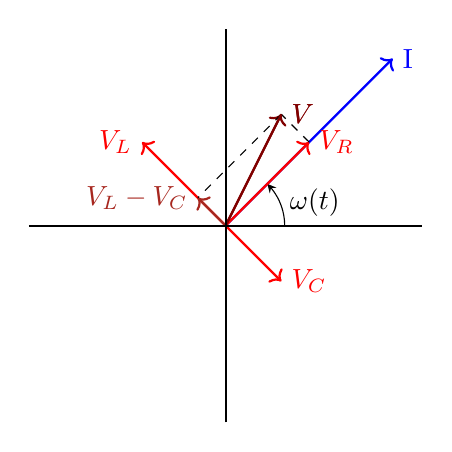
\begin{tikzpicture}
  	\draw[thick,->,Blue] (0,0) -- (45:3) node[right] {I};
  	\draw [>=stealth,->] (0.75,0) arc(0:45:0.75);
  	\draw (0,0) ++(22.5:0.75) node[right]{$\omega(t)$};
  	\draw[thick,->,Red] (0,0) -- (45:1.5) node[right] {$V_R$};
  	\draw[thick,->,Red] (0,0) -- (135:1.5) node[left] {$V_L$};
  	\draw[thick,->,Red] (0,0) -- (-45:1) node[right] {$V_C$};
  	\draw[thick,->,Mahogany] (0,0) -- (135:0.5) node[left] {$V_L - V_C$};
  	\draw[thick,->,Maroon] (0,0) -- (0.707,1.414) node[right] {$V$};
  	\draw[dashed] (0.707,1.414) -- (135:0.5);
  	\draw[dashed] (45:1.5) -- (0.707,1.414);
  	\draw[thick,>=stealth,Maroon] (0,0) -- (0.707,1.414) node[right] {$V$};
  	
  	\draw[thick] (0,-2.5) -- (0,2.5) ;
  	\draw[thick] (-2.5,0) -- (2.5,0) ;
  	
  	\end{tikzpicture}
  \end{center}

Par le diagramme des phaseurs des trois composants, on peut trouver une expression pour l'impédance
\[Z = \sqrt{R^2 + (X_L - X_C)^2} =
\sqrt{R^2 + \left(\omega{L} - \frac{1}{\omega{C}}\right)^2}\]
Le déphasage $\phi$ du courant par rapport à la tension de la source obéit quant à lui à l'équation
\[\tan{\phi} = \frac{X_L - X_C}{R} = \cfrac{\omega{L} -\cfrac{1}{\omega{C}}}{R}\]

\subsection{Application: Tuner une radio}
Les ondes radio sont des ondes électromagnétiques, elles ont donc une fréquence bien particulière. En donnant à la source la même fréquence que celle de l'onde nous obtenons un phénomène de résonance et donc un transfert d'énergie optimale. Dans les radios on va faire varier une capacité jusqu'à ce que la tension et le courant soient en phase.

	Pour qu'il n'y ait pas de décalage entre $v$ et $i$ il faut que:
	\[ \phi =0 \]
	Donc
	\[ X_L = X_C \]
	\[ \omega = \sqrt{\frac{1}{LC}}  \]

\section{Puissance}
Comme d'habitude, la puissance que transmet la source de courant alternatif en fonction du temps vaut
\[ p = vi \]
Une valeur plus intéressante est la puissance moyenne, qui dépend du déphasage $\phi$ entre le courant et la tension :
\[ P_\mathrm{av} = V_\mathrm{rms} I_\mathrm{rms} \cos\phi \]
\textbf{Attention} : $P_\mathrm{av} \neq P_\mathrm{rms}$ ! La valeur de $P_\mathrm{rms}$ n'a aucun sens physique. \\
Le facteur $\cos\phi$ est appelé \emph{facteur de puissance}. Notons trois cas importants :
\begin{description}
    \item[résistance pure] $\phi = 0$ et $P_\mathrm{av} = V_\mathrm{rms} I_\mathrm{rms}$ : le circuit se comporte comme un circuit en courant continu ;
    \item[inductance pure] $\phi = \ang{90}$ et $P_\mathrm{av} = 0$ : toute la puissance fournie à l'inductance est retournée à la source une fois que le champ magnétique est établi ;
    \item[capacité pure] $\phi = \ang{-90}$ et $P_\mathrm{av} = 0$ : toute la puissance fournie à la capacité est retournée à la source une fois que la capacité est chargée.
\end{description}

\section{Transformateur}
\label{sec:transfo}
\begin{center}
  \begin{circuitikz}[american] \draw
    (0,0) node[transformer] (T) {}
    (T.B1) -| (3.5, 0) to[R, v=$V_2$, i = $I_2$] (3.5,-2) |- (T.B2)
    (T.A1) -| (-3.5, 0) to[sV, v=$V_1$, i = $I_1$] (-3.5,-2) |- (T.A2)
    (-1,-1) node{$N_1$}
    (1,-1) node{$N_2$}
    ;
  \end{circuitikz}
\end{center}

Le transformateur respecte deux équations
\[\frac{V_1}{V_2} = \frac{N_1}{N_2}\qquad{\qquad{\qquad}}V_1I_1 = V_2I_2\]

Par la conservation du flux (voir la matière du cours LFSAB1202), on a
\[ \frac{V_1}{V_2} = \frac{N_1}{N_2} \]

Si on considère que le transformateur ne perd pas d'énergie, on a
\[ V_1I_1 = V_2I_2 \]

Attention au sens des courants, si on les définit dans l'autre sens,
les signes peuvent changer donc ce sont des égalités au signe près.

% TODO insert http://www.forum-epl.be/viewtopic.php?p=108384#108384

\section{Bloc d'alimentation}
Le rôle d'un bloc d'alimentation est de transformer un courant alternatif (venant du réseau) en un courant continu, qui sert à toutes sortes d'appareils électroniques. Il est composé de trois parties :
\begin{description}
    \item[transformateur] même principe que dans la section \ref{sec:transfo} : il sert à abaisser les très hautes tensions du réseau à des tensions plus acceptables pour l'appareil électronique ;
    \item[redresseur] à l'aide de diodes, il fait en sorte que le courant passe toujours dans le même sens dans la branche d'arrivée :
    \item[filtre] à l'aide d'une capacité, il se charge pendant que la tension alternative monte et se décharge lorsqu'elle redescend : ainsi, une tension quasi-constante est assurée aux bornes de sortie.
\end{description}

\begin{center}
    \begin{circuitikz}[american]
        \draw (0, 0)
        to[short, o-] (1, 0)
        to[L, mirror] (1, 3)
        to[short, -o] (0, 3);
        \draw (2, 0)
        to[L] (2, 3)
        to[short] (3, 3)
        to[empty diode, *-*] (6, 3)
        to[short] (7, 3)
        to[C, *-*] (7, 0)
        to[short] (6, 0)
        to[empty diode, *-*] (3, 0)
        to[short] (2, 0);
        \draw (3, 0)
        to[short] (4.5, 1.5)
        to[empty diode] (6, 3);
        \draw (6, 0)
        to[empty diode] (4.5, 1.5)
        to[short] (3, 3);
        \draw (7, 0)
        to[short] (9, 0)
        to[resistor] (9, 3)
        to[short] (7, 3);
    \end{circuitikz}
\end{center}


  \begin{center}
  	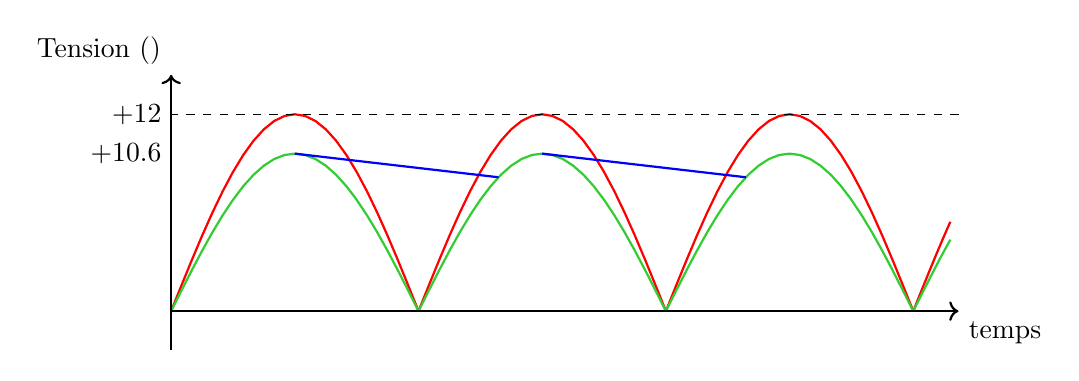
\begin{tikzpicture}

		\draw [thick,domain=0:pi,red] plot (\x,{2.5 * sin(\x r)});
		\draw [thick,domain=pi:2*pi,red] plot (\x,{-2.5 * sin(\x r)});
		\draw [thick,domain=2*pi:3*pi,red] plot (\x,{2.5 * sin(\x r)});
		\draw [thick,domain=3*pi:3.15*pi,red] plot (\x,{-2.5 * sin(\x r)});

		\draw [thick,domain=0:pi,green!60!gray] plot (\x,{2 * sin(\x r)});
		\draw [thick,domain=pi:2*pi,green!60!gray] plot (\x,{-2 * sin(\x r)});
		\draw [thick,domain=2*pi:3*pi,green!60!gray] plot (\x,{2 * sin(\x r)});
		\draw [thick,domain=3*pi:3.15*pi,green!60!gray] plot (\x,{-2 * sin(\x r)});

		\draw[thick,blue] (pi /2,2) -- (pi +1.01598529381,1.7);
		\draw[thick,blue] (3*pi /2,2) -- (2*pi +1.01598529381,1.7);

		\draw[thick,->] (0,0) -- (10,0) node[anchor=north west] {temps};
		\draw[thick,->] (0,-0.5) -- (0,3) node[anchor=south east] {Tension (\si{\volt})};
		\draw[dashed] (10,2.5) -- (0,2.5) node[left]{+12};
		\draw (0,2) node[left]{+10.6};

  	\end{tikzpicture}
  \end{center}
    
La tension rouge est la tension aux bornes du transformateur. Ensuite, la tension verte est la tension au niveau du redresseur (nous avons une chute de tension de \SI{0.7}{\volt} par diode). Finalement, la tension bleue est la tension aux bornes du filtre.

\section{Amplificateur opérationnel}

% TODO améliorer le positionnement des figures (trop de blanc)
   
% SOURCE slides de Jean-Didou

L'ampli op est un composant qui prend une tension d'entrée et l'amplifie en sortie d'un facteur $A$.

\begin{figure}[H]
    \centering
    \begin{circuitikz}[american]
    % utiliser l'option 'invert' sur la source de tension et les tensions si circuitikz change leur sens.
    \fill[cyan!50] (0, 0) -- (0, 6) -- (5, 3) -- cycle; % le triangle
    \draw (6, 0) node[ground] {}
        to[open, v<=$v_\mathrm{o}$, o-o] ++(0, 3)
        to[short, o-] ++(-5, 0)
        to[cV=$Av_{in}{=}A(v_{in+} - v_{in-})$] ++(0, -1.5)
        to[short] ++(0, -1.5) node[ground] {};
    \draw (0, 4.5) node[right] {$-$}
        to[short, i<=$i_{in-}{=}0$] ++(-3, 0)
        to[open, v=$v_{in-}{=}v_1$, o-o] ++(0, -4.5) node[ground] {};
    \draw (0, 1.5) node[right] {$+$}
        to[short, i<_=$i_{in+}{=}0$] ++(-2, 0)
        to[open, v^=$v_{in+}{=}v_2$, o-o] ++(0, -1.5) node[ground] {};
    %\draw (0, 1.5) to[open, v=$v_{in}$] (0, 4.5);
    \end{circuitikz}
\end{figure}
Le facteur d'amplification $A$ est souvent très grand ; on considère donc que la tension entre les bornes d'entrée est proche de zéro : $v_2 - v_1 = \frac{v_\mathrm{o}}{A} \approx 0$. Notons également que le courant entrant dans les branches d'entrée est nul (comme indiqué).

\subsection{Montage inverseur}
	
\begin{center}
	\begin{circuitikz}[american]
	% utiliser l'option 'invert' sur la source de tension et les tensions si circuitikz change leur sens.
	\draw
	(2, 2) node[op amp] (opamp) {}
	(opamp.+) -- ++(-0.5, 0) node[above] {$2$} -- ++(0, -0.5) node[ground] {}
	(opamp.-) to[short, -*] ++(-0.5, 0) node[below] {$1$}
	          to[R=$R_1$] ++(-2, 0)
	          to[V_=$v_1$] ++(0, -1.5) node[ground] {}
	(opamp.-) ++(-0.5, 0)
	          |- ++(0.5, 1)
	          to[R=$R_2$] ++(2, 0)
	          -| (opamp.out) node[below] {$3$}
	          to[short, *-] ++(0.5, 0)
	          to[open, v^=$v_o$, o-o] ++(0, -1) node[ground] {}
	;
	\end{circuitikz}
\end{center}

En appliquant la méthode des noeuds au point 1, on trouve la relation
\[ \frac{v_1 - 0}{R_1} = \frac{0 - v_o}{R_2} \Rightarrow \frac{v_o}{v_1} = -\frac{R_2}{R_1} \]

\subsection{Montage non-inverseur}
\begin{center}
	\begin{circuitikz}[american]
	% utiliser l'option 'invert' sur la source de tension et les tensions si circuitikz change leur sens.
	\draw
	(2, 2) node[op amp] (opamp) {}
	(opamp.+) -- ++(-0.5, 0) node[above] {$2$}
	          to[V_=$v_1$] ++(0, -1.5) node[ground] {}
	(opamp.-) to[short, -*] ++(-0.5, 0) node[below] {$1$}
	          to[R, l_=$R_1$] ++(-2, 0)
	          to[short] ++(0, -0.5) node[ground] {}
	(opamp.-) ++(-0.5, 0)
	          |- ++(0.5, 1)
	          to[R, l^=$R_2$] ++(2, 0)
	          -| (opamp.out) node[below] {$3$}
	          to[short, *-] ++(0.5, 0)
	          to[open, v^=$v_o$, o-o] ++(0, -2) node[ground] {}
	;
	\end{circuitikz}
\end{center}

La tension à la borne négative vaut pratiquement $v_\mathrm{I}$ ; on pose le sens du courant de droite à gauche et on applique encore la méthode des n\oe{}uds à la borne négative.
\[ \frac{v_o - v_1}{R_2} = \frac{v_1 - 0}{R_1} \Rightarrow \frac{v_o}{v_1} = 1+\frac{R_2}{R_1} \]

\subsection{Montage intégrateur}
\begin{center}
	\begin{circuitikz}[american]
	% utiliser l'option 'invert' sur la source de tension et les tensions si circuitikz change leur sens.
	\draw
	(2, 2) node[op amp] (opamp) {}
	(opamp.+) -| ++(-0.5, -0.5) node[ground] {}
	(opamp.+) ++(-0.5, 0) node[above] {$2$}
	(opamp.-) to[short] ++(-0.5, 0) node[below] {$1$}
	          to[R, l_=$R$] ++(-2, 0)
	          to[V_=$v_1$] ++(0, -1.5) node[ground] {}
	(opamp.-) ++(-0.5, 0)
	          |- ++(0.5, 1)
	          to[C=$R$] ++(2, 0)
	          -| (opamp.out) node[below] {$3$}
	          to[short, *-] ++(1, 0)
	          to[open, v^=$v_o$, o-o] ++(0, -1) node[ground] {}
	;
	\end{circuitikz}
\end{center}

Nous savons que la tension au n\oe{}ud 1 est de 0 donc:
\[ \frac{v_1}{R} = -C\frac{\dif v_o}{\dif t} \Rightarrow v_o(t) = -\frac{1}{RC} \int v_1(t) \dif t \]

\subsection{Montage différenciateur}
\begin{center}
	\begin{circuitikz}[american]
	% utiliser l'option 'invert' sur la source de tension et les tensions si circuitikz change leur sens.
	\draw
	(2, 2) node[op amp] (opamp) {}
	(opamp.+) -| ++(-0.5, -0.5) node[ground] {}
	(opamp.+) ++(-0.5, 0) node[above] {$2$}
	(opamp.-) to[short] ++(-0.5, 0) node[below] {$1$}
	          to[C, l_=$C$, *-] ++(-2, 0)
	          to[V_=$V_1$] ++(0, -1.5) node[ground] {}
	(opamp.-) ++(-0.5, 0)
	          |- ++(0.5, 1)
	          to[R=$R$] ++(2, 0)
	          -| (opamp.out) node[below] {$3$}
	          to[short, *-] ++(1, 0)
	          to[open, v^=$v_o$, o-o] ++(0, -1) node[ground] {}
	;
	\end{circuitikz}
\end{center}
    \[ C\frac{\dif v_1}{\dif t} = -\frac{v_o}{R} \Rightarrow v_o(t) = -RC \frac{\dif v_1(t)}{\dif t} \]

\subsection{Montage sommateur}

\begin{center}
	\begin{circuitikz} [american]
		\draw %Ampli
		(2,2) node[op amp] (opamp){}
		(opamp.+) node[left] {}
		(opamp.-) node[left] {}
		(opamp.out) node[right] {}
		
		(6.5,1.51) node[op amp] (opamp2){}
		(opamp2.+) node[left] {}
		(opamp2.-) node[left] {}
		(opamp2.out) node[right] {};
		\draw (-2.5,1.49)
		to[resistor=$R_2$,o-*] (-1, 1.49)
		to[short] (-0.5,1.49)
		to[short] (-0.5,2.49);
		\draw (-2.5,2.49)
		to[resistor=$R_1$,o-*] (-1, 2.49)
		to[short] (-0.5,2.49)
		to[short] (0.5,2.49)
		to[short] (0.5,3.5)
		to[R=$R_a$] (3,3.5)
		to[short,-*] (3, 2)
		to[R=$R_b$](4.5,2)
		to[short,-*](5,2);
		\draw(3,1)
		to[R=$R_3$,o-] (4.5,1)
		to[short](5,2);
		\draw(3,0)
		to[R=$R_4$,o-] (4.5,0)
		to[short](5,2);
		\draw (5.67,2)
		to[short] (5,2)
		to[short](5,3)
		to[R=$R_c$] (7.5,3)
		to[short, -*] (7.5,1.5)
		to[short] (8,1.5);
		\draw(1, 2.49) %ampli - 1
		to[short] (0.5, 2.49);
		\draw (1.17, 1.51)% borne + ampli
		to[short] (0.5, 1.51)
		to[short](0.5,1)
		node[ground]{};
		\draw (5,0)
		node[ground] {}
		to[short] (5,1.02)
		to[short] (5.67,1.02);
		\draw 
		(-2.9,1.49) node[] {$v_1$}
		(-2.9,2.49) node[] {$v_2$}
		(2.6,1) node[] {$v_3$}
		(2.6,0) node[] {$v_4$}
		(0.5,2.25) node {1}
		(0.5, 1.7) node {2}
		(3,1.75) node {3}
		(8.05,1.485) node[ocirc]{}
		(8.4,1.485) node[] {$v_o$};
	\end{circuitikz}
\end{center}

La tension de sortie du premier ampli vaut (au n\oe{}ud 3)
\[ v_{o1} = -R_a (\frac{v_1}{R_1} + \frac{v_2}{R_2}) \]
Le courant passant dans la résistance $R_b$ vaut donc
\[ i_b = \frac{v_{o1}}{R_b} \]
Dans le cas où $R_a = R_b$ (et uniquement dans ce cas !), on a
\[ i_b = - \left(\frac{v_1}{R_1} + \frac{v_2}{R_2} \right) \]
Enfin, la tension de sortie vaudra
\[ v_o = -R_c \left(i_b + \frac{v_3}{R_3} + \frac{v_4}{R_4}\right) = R_c \left(\frac{v_1}{R_1} + \frac{v_2}{R_2} - \frac{v_3}{R_3} - \frac{v_4}{R_4} \right) \]

\end{document}
